\documentclass[a4paper,12pt, draft]{report} 

\usepackage[francais]{babel}
\usepackage[utf8]{inputenc}
\usepackage[T1]{fontenc}
\usepackage[tight]{shorttoc}
\usepackage{color}
\usepackage[final]{pdfpages}


\author{Bérenger Ossete Gombe}
\title{Dossier Projet Professionnel}
\date{Décembre - Janvier 2015}

%==================== NEW COMMANDS ====================
%\newcommand{\tabTitle}[1]{\multicolumn{1}{|c|}{\textsc{#1}} }
\newcommand{\tabTitle}[1]{\hfill{} \textsc{#1} \hfill{} }
\newcommand{\sommaire}{\shorttoc{Sommaire}{1}}
\newcommand{\bogCitation}[2]
{
  \begin{quote}
    ``#1''
  \end{quote}

  \begin{flushright}
    \bsc{#2}
  \end{flushright}
}
\newcommand{\goodPoint}[1]{\textcolor{green}{\textbf{\textit{#1}}}}
\newcommand{\badPoint}[1]{\textcolor{red}{\textbf{\textit{#1}}}}
\newcommand{\importantPoint}[1]{\textcolor{blue}{\textbf{\textit{#1}}}}
%======================================================

\begin{document}
\maketitle

\newpage
\sommaire{}

\newpage

\part{Introduction}

\chapter{Remerciements}
\paragraph{}
Je tiens à remercier mes enseignants et en particulier Fabien \textsc{Peureux} et Hélène \textsc{Gouillardon}. Les cours d'Atelier Projet Professionnel et de Projet Personnel et Professionel m'ont grandement aidé à la rédaction de ce dossier jusque dans sa structure \textsc{bilan-projet-marché-action}.

\paragraph{}
Merci également à mon ami Ervan \textsc{Silvert} pour m'avoir fait découvrir \LaTeX\ et pour avoir mis à ma disposition son dossier PPP afin de m'aider avec ce nouvel outil.

\paragraph{}
Merci enfin aux volontaires ayant donné leur temps pour une interview improvisée: Alain \textsc{Giorgetti}, Céline \textsc{Libéral}, \textsc{Chriswot} et \textsc{Yakulu}.

\chapter{Guide de lecture}
\paragraph{}
Ce dossier est composé de trois grandes parties: le bilan personnel, le projet professionnel et les stratégies d'actions. Dans le sujet, la partie bilan est traitée après le projet. J'ai décidé d'inverser cela car chronologiquement, le bilan personnel est antérieur à l'établissement du projet professionnel.
Je me suis beaucoup aidé des ressources disponibles sur \textsc{moodle}: à commencer par la structure du rapport.

\paragraph{}

\part{Bilan personnel}

\chapter{Compétences et savoirs} 

Dans ce chapitre, nous allons faire une synthèse de mes compétences.
Celles-ci seront traitées selon leur nature.
Étant issues de savoirs différents, j'ai décidé de les traiter en deux parties.


\section{Introspection}
Dans cette partie, nous allons nous intéresser aux compétences liées au \textbf{savoir-être} et à la \textbf{personnalité}. Celle-ci est consituée de traits que l'on peut considérer comme des qualités ou bien comme des défauts. Il est alors difficile de rester objectif tant cela est une affaire de \textbf{point de vue}. Je m'appréhende d'une certaine manière, les autres me voient différemment, et la perception varie en fonction du regard des autres. Cette divergence des points de vues rend mon travail d'analyse tout à fait \textbf{subjectif}. Je traiterai ici uniquement ma vision que je m'efforcerai de pondérer en m'aidant d'un exercice d'autoportrait\footnote{Voir en Annexe \ref{autoportrait} en page \pageref{autoportrait}} effectué dans le cadre du CMI\footnote{Cursus Master en Ingénierie}.

\newpage
\subsection{Comportement}

Voici en premier lieu un classement de ce que j'estime être mes principaux traits de personnalité. Je ne les qualifie volontairement pas de défauts ou de qualités.\\

\begin{description}
\item [Curieux]car j'adore apprendre et découvrir de nouvelles choses.
\item [Partageur]car j'aime recevoir autant qu'offrir et je crois en la coopération.
\item [Volontaire]car j'aime relever des challenges, aller plus loin et appronfondir.
\item [Timide]car j'aime me retrouver dans des situations connues et/ou maîtrisées
\item [Perfectionniste]car je refuse l'abandon et l'échec.
\item [Rêveur]car j'aime suivre mon instinct et mes envies.
\end{description}

\begin{table}[h]
  \begin{tabular}{|l|c|c|}
    \hline

  \tabTitle{Trait} & \multicolumn{2}{c|}{\tabTitle{Point de vue}} \\
\hline
 & \tabTitle{Qualité} & \tabTitle{Défaut} \\
\hline
  Curieux & Passionné & Trop agité, éparpillé \\
  \hline
  Partageur & Sociable & Dépendant\\
  \hline
  Volontaire & Dynamique & Entêtement \\
  \hline
  Timide & Réfléchi & à l'écart des autres \\
  \hline
  Perfectionniste & Appliqué & Obsédé \\
  \hline
  Rêveur & Imaginatif & Dispersé \\
  \hline


    
  \end{tabular}\\
\caption{Approche de mes principaux traits de personnalité}
\end{table}


\subsection{Motivations}
Mes principales motivations sont  l'\textbf{acquisition de savoirs} et 
le \textbf{partage de connaissances}. 

\paragraph{L'attrait pour la curiosité}
\subparagraph{}
Depuis toujours j'ai été attiré par ce qui est nouveau, étonnant et différent de ce que je connais d'habitude.
\subparagraph{Exemple}
J'ai une certaine connaissance du C++, qui est un langage de programmation que je n'ai pas vu dans le cadre de mes études.  Ce que je sais et ce que je suis capable de faire en algorithmique et à l'aide du C++, je l'ai acquis seul, à l'aide de cours et tutoriels trouvés sur l'internet. 

 

\paragraph{L'importance du partage}
\subparagraph{}
Tout ce que j'ai appris en dehors de mes études est principalement dû à l'internet et aux projets d'éducation pour tous tels Wikipedia ou OpenClassRooms\footnote{Anciennement ``le site du zéro''}.
Je soutiens totalement ce genre de projets qui, je le pense, sont dans l'esprit du siècle des lumières avec leurs idéaux de diffusion du savoir. Le partage du savoir permet à tout le monde d'accéder à la connaissance en toute liberté et sans discrimination. Cela m'a permis de découvrir, de me renseigner, d'apprendre. 

\subparagraph{}
La découverte apparaît alors comme une première étape, le partage de cette même découverte étant la seconde. Je pense que le partage est nécessaire, et que sans partage, on aboutit rapidement  à l'établissement d'une élite intellectuelle. Si le savoir n'est pas partagé, alors on entre dans un modèle de confrontation entre ceux qui détiennent le savoir (qui manipulent) et les autres (qui tentent de se libérer). Je pense que la coopération est le modèle le plus profitable pour tous.

\subparagraph{Exemple} En terminale j'ai fait découvrir à mon meilleur ami la programmation en C++. Il s'est par la suite redirigé vers un cursus informatique (ce qui me permet de croire que mon partage a été concluant et efficace).




\subsection{Valeurs}
\paragraph{}
Nous avons vu que mes principales motivations sont l'acquisition de\\ connaissances puis leur partage. Derrière ces motivations, se cachent des valeurs.
Mes valeurs tournent autour du respect de la \textbf{liberté} et du \textbf{bon sens}.

\paragraph{Ma découverte du libre}

Ma première expérience de la liberté informatique concerne le site web Wikipédia. J'ai été émerveillé par cette Encyclopédie moderne.
Ce projet collaboratif permet à tout le monde d'apprendre et de participer à la diffusion des connaissances.
J'ai ensuite fait connaissance avec l'OS\footnote{\textsc{OS}: Operating System (Système d'exploitation)} Gnu/Linux par pur hasard. J'ai fait alors l'expérience d'une liberté que je ne connaissais pas avec Windows. J'utilisais toujours ce dernier, considérant Gnu/Linux comme une curiosité technologique intéressante. 
Cela a duré jusqu'au moment où je suis tombé par pur hasard (encore une fois) sur une conférence de R.Stallman\footnote{Richard Matthew \textsc{Stallman} (1953 - ): Fondateur de la Free Software Foundation et diffuseur historique des idées du logiciel libre.}. J'ai alors réalisé à quel point la liberté était importante pour moi.

%\paragraph{L'influence du libre sur moi}
%Je suis convaincu que nous devons avoir des logiciels libres, tournant sur du materiel libre et en communication entre eux via des bandes-passantes libres afin de rester maître de notre informatique.
%C'est un combat qui me tient à coeur car il me parait juste, éthique et d'une importance capital dans la mesure où nous construisons une ``société assistée par ordinateur''. Je suis en faveur d'une informatique libre, et également d'une culture libre et d'une éducation libre. En effet, je pense que l'homme devrait être au centre de la société en tant qu'acteur et non en tant que produit. Le savoir devrait être partagé, et non breveté, caché et vendu sous licence.

\paragraph{}
Mes motivations sont donc portées par ces valeurs. Celle-ci guident grandement la construction de mon projet professionnel, c'est pourquoi j'ai pris la liberté d'autant les détailler.
Je vais ainsi devoir accorder ces valeurs avec mon projet professionnel, ce qui constitue une \textbf{très forte contrainte} que je me fixe comme nous le verrons dans la synthèse du bilan personnel \footnote{Voir le chapitre \ref{RefSyntheseBilanPerso} en page \pageref{RefSyntheseBilanPerso}}.

\newpage

\section{Compétences métiers}
\subsection{Ma formation}
Voici la liste des diplômes\footnote{Licence d'informatique à venir} obtenus au cours de ma scolarité.
\begin{table}[h]
\begin{center}
\begin{tabular}{|l|c|r|}
\hline
\tabTitle{Diplôme} & \tabTitle{Années} & \tabTitle{Établissement}\\
\hline
Brevet des collèges & 2010 & Collège Joseph Proudhon \\
\hline
Baccalauréat Scientifique & 2013 & Lycée Louis Pasteur \\
\hline
Licence d'Informatique & 2016 & Université de Franche-Comté\\
\hline
\end{tabular}
\end{center}
\caption{Diplômes obtenus} 
\end{table}

\subsection{Mon expérience}
\paragraph{}
Je n'ai \textit{\textbf{aucune}} expérience professionnelle en dehors de mon stage de troisième.

\paragraph{}
Durant cette année de L2, j'ai pu participer à plusieurs reprises à des \textbf{événements organisés par l'Université de Franche-Comté}. Ces événements m'ont apportés des expériences de travail d'équipe. En voici un résumé.

\begin{table}[h]
\begin{tabular}{|l|c|l|}
\hline
\tabTitle{Expérience}  &  \tabTitle{Contexte} & \tabTitle{Technologies}\\
\hline
Nuit de L'info 2014  & UFC & Javascript/WebGL\\
\hline
Club jeux-vidéo (DPS\footnotemark{})  & UFC & C++/SFML 2.1\\
\hline
\end{tabular}
\caption{Expériences scolaires}
\end{table}
\footnotetext{Dead Pixel Society- Club de jeux vidéo de l'UFC}

\chapter{Synthèse} \label{RefSyntheseBilanPerso}
Nous avons vu précédemment une liste de mes compétences et de mes savoirs.
En voici une synthèse.

\paragraph{Savoir}
J'ai un baccalauréat scientifique et je prépare une licence d'informatique.
Je suis actuellement en L2.

\paragraph{Savoir-Être}
Je suis intéressé par la découverte et le partage de connaissances. C'est un de mes points forts car je suis très motivé et volontaire.

\paragraph{Savoir-Faire}
Il s'agit véritablement de mon point faible car je ne possède aucune expérience (ni professionnelle ni extra scolaire).

\section{Mes objectifs}
Mon objectif principal est d'apprendre, d'acquérir de nouvelles compétences au sein d'un travail.
\section{Mes priorités}
\paragraph{}
Dans le cadre du module de PPP, j'ai fait un travail d'analyse sur mes priorités professionnelles. Voici les trois plus importantes.


\paragraph{Mes priorités professionnelles}
\begin{enumerate}
\item Travailler dans un milieu professionnel qui correspond à mes valeurs
\item Pouvoir faire preuve de créativité
\item Développer mes compétences : actualiser mon potentiel
\end{enumerate}


\paragraph{}
\subparagraph{Travailler dans un milieu professionnel qui correspond à mes valeurs}
Car je ne pense pas être capable de travailler dans un milieu ayant des valeurs trop différentes des miennes. 

\subparagraph{Pouvoir faire preuve de créativité}
Car je trouve qu'il est important pour moi d'avoir un degré de liberté minimum. En effet, la possibilité de faire preuve de créativité permet de personnaliser, d'adapter et d'orienter son travail.

\subparagraph{Développer mes compétences : actualiser mon potentiel}
Car j'aime apprendre de nouvelles choses et m'améliorer, et que je ne souhaite pas stagner professionnellement.

\chapter[Mon projet idéal]{Vers un projet professionnel: mon projet idéal}
Il s'agit ici de définir ce que je \textsc{\textbf{veux}} faire sans s'occuper de ce que je peux faire (nous nous occuperons de cela dans la construction du projet) en fonction de ce que je suis, ce que j'ai fait et ce que je sais faire.


\begin{table}[h]
\begin{center}
\begin{tabular}{|l|c|c|}
  \hline
  \tabTitle{activité} & \tabTitle{attrait} & \tabTitle{inconvénient}\\
  \hline
  \hline
  L'enseignement & le partage & pas assez technique\\
  \hline
  La recherche & la curiosité & néant \\
  \hline
  Les SSII\footnotemark{}/SSLL\footnotemark{} & le libre & trop rare\\
  \hline
  Développeur & travail d'équipe & peu créatif\\
  \hline
  La création d'activité & tout & risqué\\
  \hline
\end{tabular}
\end{center}
\caption{Ce que je veux faire}
\end{table}

\footnotetext[1]{\textsc{SSII}: Société de Service en Ingénierie Informatique (également SS2I) }
\footnotetext[2]{\textsc{SSLL}: Société de Service en Logiciel Libre (également SS2L) }


\begin{description}
\item [Enseignement] C'est ce qu'il y a de mieux pour partager sa passion pour l'informatique. Malheureusement, je trouve ça trop peu technique: on passe \textbf{tout} son temps à enseigner et donc on n'a pas le temps d'approfondir véritablement.

\item [Recherche] Semble correspondre parfaitement avec mes motivations et\\ valeurs.

\item [Les SSII] Intéressant car on change souvent de client ce qui permet de varier son travail. Cependant travailler pour un SS2I me forcerait potentiellement à devoir travailler avec des outils non-libres et pour des sociétés qui pourraient ne pas être en phase avec mes valeurs.

\item [Les SSLL] Même intêret que pour les SS2I, les éventuels conflits de valeurs en moins. Ces sociétés sont relativement rares\cite{annuaire_ssll}, ce qui m'obligerait à me déplacer.
 
\item [Création d'activité] Cela me semble très intéressant mais également très risqué. Cependant, je pense qu'il y a des choses à faire du coté logiciel libre.

\item [Développement] Intuitivement je dirais que ça m'intéresse beaucoup. \\J'aime le travail d'équipe et j'aime programmer. Cependant ça risque de ne pas me convenir pour le coté routinier du métier. Je pense également ne pas apprécier de \textit{faire} sans \textit{concevoir}.
\end{description}


\part{Projet Professionnel}

\chapter{Construction du projet}
\paragraph{}
Dans la partie finale du bilan personnel, j'ai dégagé plusieurs projets qui me plairaient d'entreprendre. Cependant, je vais devoir un choisir un. Devant cette difficulté, je choisis de me lancer dans le projet le plus général et le plus en phase avec mon parcours scolaire: \tabTitle{\fbox{la recherche}}. \\

\paragraph{}
J'ai choisi ce projet professionnel car il me laisse la possibilité de changer plus tard. Il me laisse le temps de découvrir des domaines de l'informatique que je ne connais pas\footnote{le web, le réseau, les systèmes embarqués...}. 

\paragraph{}
Initialement, ce projet me motivait et m'intéressait beaucoup, mais en me renseignant, j'ai découvert que \textit{je me faisais une idée fausse du métier de chercheur}. Je détaillerai ce point en conclusion de cette partie.



\chapter{Rencontre avec un professionnel}
\paragraph{}
Afin d'appuyer mon choix de projet professionnel, j'ai contacté des personnes travaillant dans les domaines qui m'intéresse.
J'ai donc discuté avec trois personnes en irc\footnote{\textsc{IRC}: Internet Relay Chat ou IRC (en français, « discussion relayée par Internet ») est un protocole de communication textuelle sur Internet .} et j'ai rencontré un enseignant-chercheur de l'université de Franche-Comté.

\paragraph{}
N'étant pas sûr de mon projet professionnel, les trois premières interview m'ont permis d'avoir \textbf{un aperçu de mes possibilités et de mes envies.} Celles-ci n'étaient initialement pas prévues et encore moins préparées. Je les ai incluses dans ce dossier pour l'aide qu'elles m'ont apporté.
Pour ces raisons, je ne connais presque rien de mes interlocuteurs: je connais uniquement leurs pseudos et leurs professions.

\paragraph{}
La dernière interview est la plus importante: il s'agit d'une rencontre avec un enseignant-chercheur autour de la recherche. Mon projet professionnel étant plus net dans mon esprit au moment de notre rencontre, j'ai pu poser des questions préparées et pertinentes (contrairement aux précédentes entrevues).

\paragraph{}
Voici la notation utilisée dans les interviews:
\begin{description}
\item [Question]: Voici la question que je pose.
\item [Réponse]: Et voici la réponse de mon interlocuteur. Dans les réponses, je vais apprendre des choses qui seront (ou non) en phase avec mon projet professionnel. En effet, je mettrai en avant ce qui me semble \importantPoint{important}, \goodPoint{bien}, et ce qui me semble \badPoint{mauvais}.
\end{description}


\section{Présentations}
\subsection[Un membre de Framasoft]{Un membre de Framasoft\footnote{\textsc{framasoft}: Association française de loi 1901, issue du monde éducatif, Framasoft est un réseau d'éducation populaire consacré principalement au logiciel libre. }: \fbox{Yakulu}}
Fabien, alias Yakulu, est un membre de l'association Framasoft. Fabien est entrepreneur-salarié dans une coopérative d'activités \footnote{\textsc{Coopérative d'activité}: Les coopératives d'activités et d'emploi (CAE) constituent un concept original permettant à un particulier de tester une production ou un service en toute sécurité.

L'originalité de la CAE est d'offrir au porteur de projet un statut "d'entrepreneur salarié" qui lui permet de percevoir un salaire et de bénéficier de la couverture sociale d'un salarié classique.} et d'emploi.

\subsection[Un contributeur du projet LibreOffice]{Un contributeur du projet LibreOffice: \fbox{Chriswot}}
Chriswot est un contributeur de LibreOffice australien.

\subsection[Une développeuse de jeux vidéo]{Une développeuse de jeux vidéo: \fbox{Céline Libéral}}
Céline Libéral possède le ``studio''\footnote{Je ne sais pas comment appeler ça autrement: Célisoft possède une structure juridique.} de jeu libre Célisoft qu'elle a fondé en juin 2014. Elle a travaillé pour des entreprises françaises avant de se lancer à son propre compte.

\subsection[Un enseignant-chercheur]{Un enseignant-chercheur: \fbox{Alain Giorgetti} }
Alain Giorgetti est enseignant-chercheur à l'Université de Franche-Comté. Il est membre de l'équipe de recherche \textsc{Vesontio}\footnote{Vérification et Validation de logiciels et de systèmes embarqués}.\\

\begin{tabular}{c|c}

    Tél. & 03 81 66 66 60\\
\hline
    Courriel & agiorget@femto-st.fr\\
\hline
    Site personnel & http://members.femto-st.fr/alain-giorgetti/\\

\end{tabular}

\section{Le libre}
\paragraph{}
Il s'agit de ma première piste de projet professionnel. Ma découverte du libre a changé ma vision de l'informatique et de ses enjeux, ce qui explique pourquoi je me suis initialement dirigé vers les métiers du libre. Ces interviews sont rapides et peu ordonnées.

\paragraph{}
Mon objectif était de me renseigner auprès des professionnels en allant leur parler directement. Pour ce faire, je me suis simplement rendu sur leur canal irc et j'ai demandé s'il y avait quelqu'un pour discuter avec moi des métiers du libres. 

\paragraph{}
Deux \textbf{volontaires} sont alors intervenus: Chriswot, un contributeur de LibreOffice et Fabien alias Yakulu, un membre de l'association Framasoft.


\subsection{L'interview de Yakulu}

\begin{description}
\item [Question]:  Bonjour ! Je prépare un dossier dans le cadre de mes études et j'aimerais discuter dix petites minutes avec un développeur. Je m'intéresse au libre et j'aimerais en faire mon métier mais je connais peu le domaine et j'aimerais connaître mes possibilités. Quelqu'un qui travaille dans le domaine du libre pour m'éclairer ?
\item [Réponse]:  Que veux-tu savoir ?
\item [Question]:  Comme j'aimerais faire du libre mon métier, j'aimerais avoir un retour d'expérience d'un développeur ayant fait ce parcours.
\item [Réponse]:  En fait, ça dépend du contexte : tu veux te lancer à ton compte, trouver du travail ? Tu souhaites créer du logiciel libre ou contribuer ou seulement utiliser ? \goodPoint{Aujourd'hui 90\%, au moins, des agences Web, la plupart des sociétés d'informatique, emploient du logiciel libre} mais \badPoint{rarement exclusivement} (et très rarement y contribuent)
\item [Question]:  Utiliser c'est sûr et certain. Contribuer et créer me conviennent tous deux.
\item [Réponse]:  Il y a des ENL (entreprise du numérique libres), parfois regroupées en clusters régionaux, qui sont sensées faire majoritairement du logiciel libre et contribuer. Le cnll\cite{cnll} les regroupe. Il y en a dans à peu près toutes les régions. Il y a des sociétés qui sont adhérentes à l'april, à des groupes d'utilisateurs locaux qui font souvent du libre. En somme, tu peux très bien faire du développement, Web ou pas, et te faire recruter par ce genre de société. Il y a même un site\cite{lolix} d'offres d'emplois spécialisées sur du logiciel libre (mais il n'est clairement pas exhaustif).
\item [Question]:  En fait, moi je m'intéresse au développement logiciel mais je ne veux pas travailler avec des outils propriétaires par choix personnel.
\item [Réponse]:  Honnêtement, si c'est surtout une histoire d'environnement de travail, tu peux trouver même dans des sociétés qui ne font pas spécifiquement du libre. Faire du logiciel libre, y contribuer dans son métier est un peu plus difficile, car \badPoint{il y a peu de sociétés, dans la globalité, qui contribuent} (alors que beaucoup utilisent). Mais si tu es compétent, il n'y a aucune raison que tu ne trouves pas dans une société spécialisée en logiciels libres: les bons développeurs restent une ressource rare, donc appréciée !
\item [Question]:  Après, moi, je m'intéresse particulièrement à l'intelligence artificielle, à la logique et au jeu vidéo.
\item [Réponse]:  Après ça dépendra notamment du lieu où tu vis, des technologies sur lesquelles tu vas te former et te spécialiser. Je connais pas très bien ces domaines, mais intuitivement je penserais que tu as plus de chances de trouver un environnement libre voire d'y contribuer en IA qu'en jeu vidéo.
\item [Question]:  Pour mon projet professionnel, j'ai plus ou moins trois gros choix: l'enseignement et/ou la recherche, l'entreprise ou la création d'activité 
\item [Réponse]:  Que ce soit console ou pc, l'immense majorité du développement de jeux nécessite des systèmes et outils fermés, du moins c'est ce qu'il me semble
\item [Question]:  Oui, c'est aussi ce que j'ai constaté. C'est pourquoi pense faire du jeu vidéo dans mon temps libre. Mais je ne sais pas trop où chercher pour ce qui est des entreprises.
\item [Réponse]:  Je t'ai donné quelques liens au dessus: le cnll regroupe plus d'une dizaine d'associations régionales qui elles-mêmes ont des dizaines de sociétés spécialisées dans le libre. De même, tu peux regarder les personnes morales adhérentes à l'APRIL, à l'AFUL, voir les offres d'emploi sur Lolix et ailleurs.

\item [Question]:  Est ce que les SSII sont exclusivement tournées vers un type de logiciel ?
\item [Réponse]:  chaque SSII ou SSLL a sa propre stratégie, y en a des spécialisées en effet
\item [Question]: Tout d'abord merci pour tes liens et tes éléments de réponses ! Comme je l'ai dit, je rédige un dossier sur mon projet professionnel (dans le cadre de mes études en informatique), puis-je reprendre notre conversation dans mon dossier ?  Afin de réutiliser notre conversation, j'aimerais ton accord. Et peux-tu rapidement te présenter Yakulu ? (Profession et/ou rôle au sein de framasoft).

\item [Réponse]:  Oui, tu peux, mais je n'ai aucune prétention d'être expert sur le sujet.  Fabien, je suis entrepreneur-salarié dans une coopérative d'activités et d'emploi (j'ai ma propre activité, comme si j'étais à mon compte)
\item [Question]:  Une coopérative d'activités ?
\item [Réponse]:  Oui, voir apce\cite{apce}
\item [Question]:  Je me rends compte que j'utilise le tutoiement depuis le début, ça ne gène pas ? (Désolé, sur internet j'ai l'habitude de tutoyer).
\item [Réponse]:  Non, dans le libre, on se tutoie tous ;)
\item [Question]:  Tu joues un rôle dans framasoft ?
\item [Réponse]:  Je suis membre de Frama. On sort tout juste de l'Assemblée Générale 2014 :)
\item [Question]:  En tant que membre, tu contribues aux divers projets ? (Je ne connais pas très bien la structure de framasoft.)
\item [Réponse]:  Je contribue essentiellement aux échanges internes, à la technique, je devrais être amené à travailler autour de framapad & framacalc.
\item [Question]:  Par technique, tu entends développement ?
\item [Réponse]:  Non, infrastructure technique, serveur etc. Framasoft ne fait pas ou peu de développement mais on a des participants ou membres qui en font à titre personnel.
\item [Question]:  Si j'ai bien compris, Framasoft offre surtout des services libres (framadate farmacalc etc).
\item [Réponse]:  Historiquement, Framasoft offrait surtout un annuaire de logiciels libres, puis s'est diversifié autour de tas de projets menés par des bonnes volontés. Aujourd'hui, il est surtout visible par ses services en ligne. Quand tu vas sur la page d'accueil\footnote{http://framasoft.org/}, tu retrouves tous les projets actifs par catégorie.
\item [Question]:  Mais les membres actifs dans le développement sont tous bénévoles ? J'ai cru voir qu'il y avait quelques permanents.
\item [Réponse]:  Il y a deux permanents. Ils gèrent surtout les projets, les coordonnent, font l'administratif et parlent de l'association envers le public (conférences, presse etc). Ils font un peu de technique aussi, essentiellement de l'adminisatrion système, mais les projets reposent quasi tous sur le bénévolat.
\item [Question]:  Donc moi qui cherche un emploi du coté du développement libre j'ai plutot interêt à regarder vers les entreprises qui utilisent le libre ?
\item [Réponse]:  Oui, \importantPoint{aucune association n'emploie de développeur à ma connaissance}, il faut aller du côté des sociétés spécialisées existantes, ou monter ta société.
\item [Question]:  Tu crois que tu pourrais me parler de ces entreprises ?
\item [Réponse]:  Il y en des centaines, difficile d'en faire des généralités. Il y a une catégorisation qui est faite dans les docs que je viens de te citer. Le mieux pour avoir des infos reste de contacter ces fédérations d'entreprises du libre, comme la cnll. Tu es dans quel coin de la france ?
\item [Question]:  D'accord (tes liens vont m'être très utiles). Tu as ta propre activité, comment et  pourquoi as-tu décidé de le faire ? (Je suis en franche-comté (donc pas grand chose ici)).
\item [Réponse]:  Il y a une étude\cite{cnll_etude} qui va t'intéresser. J'ai décidé de créer mon activité parce que je voulais travailler sur du logiciel libre, pour des associations et être en accord avec mes valeurs. Je ne suis pas sûr que mon parcours soit hyper pertinent mais j'ai encore un lien\cite{linuxfr_new} pour toi :)
\item [Question]:  Ton parcours peut m'intéresser car je pars du même stade: l'envie de travailler sur du logiciel libre et d'être en accord avec mes valeurs !
\item [Réponse]:  Il a fait une série de dépêches sur linuxfr au sujet de vivre du logiciel libre et a interviewé 5 ou 6 entrepreneurs du libre qui se sont lancés. Je vais devoir te laisser, mais n'hésite pas.
\item [Question]:  Merci beaucoup pour tous tes liens et pour avoir partagé ton expérience avec moi !
\item [Réponse]:  je t'en prie, bon courage
\item [Question]:  Et merci d'avoir donné de ton temps. Bonne continuation !
\item [Réponse]:  Merci.
\end{description}
\newpage
\subsection{Bilan}
\paragraph{Ce que j'ai appris}
Premièrement, si je veux travailler dans un environnement utilisant le logiciel libre, je peux me tourner vers le web. Cependant, peu d'entreprises utilisent \textit{exclusivement} du libre. Les associations me paraissaient intéressantes car généralement plus engagées vers le libre, mais d'après Fabien aucune association n'emploie de développeurs. Cela concorde avec mes recherches sur le sujet: le développement dans les associations est quasi-uniquement assuré par des bénévoles.
Ce que je retiens donc de cette interview est que les entreprises entièrement libres sont plutôt rares. \textbf{Le web est donc une piste intéressante}.


\subsection{L'interview de Chriswot}
Chriswot étant anglophone, cet interview à initialement été faite en anglais. Ceci est donc une traduction que je propose. L'originale est disponible en annexe\footnote{Page \pageref{chriswot_en}}.
\begin{description}
\item [Question]:  Bonjour, et merci !
\item [Réponse]:  Que veux-tu savoir ?
\item [Question]:  Je suis un étudiant en informatique et je cherche des informations au sujet du développement de logiciel libre. Je voudrais travailler dans ce domaine, mais je ne connais pas les métiers qui sont en accord avec la philosophie du logiciel libre.
\item [Réponse]:  Ça dépend - pour être payé pour faire du logiciel libre, \importantPoint{tu vas avoir besoin de trouver un job qui te paye pour faire de la maintenance.}
\item [Question]:  Ma première question serait: qui es-tu ? Un développeur du projet LibreOffice ? (Pourrais-tu te présenter ?)
\item [Réponse]:  Je suis un développeur de LibreOffice. Je suis sur le point de décrocher un contrat avec Collabora. Je travaille sur LibreOffice depuis environ un an. Je fais beaucoup de relecture et de refractoring. Je commence à connaître les gens sur l'irc petit à petit.
\item [Question]:  D'après toi, quel domaine de l'informatique est le plus concerné par le logiciel libre ?
\item [Réponse]:  Coder et tester. C'est une vaste question ! Tu veux dire, par quels aspects des logiciels je suis intéressé ? Genre les applications, les environnements de travail, les systèmes d'exploitations, etc ?
\item [Réponse]:  Et bien, pour l'instant, je m'intéresse aux applications, mais c'est un vaste domaine. Pour l'instant, je bosse sur la couche widget de LibreOffice (ça s'appelle VCL).
\item [Question]: Peux-tu m'expliquer comment est-ce que tu es entré dans le développement de logiciel libre ?
\item [Réponse]:  J'ai commencé par lire du code après avoir vu un article sur LibreOffice sur Hacker New.
\item [Question]:  Et quels conseils donnerais-tu à un étudiant voulant travailler sur du logiciel libre ?
\item [Réponse]: Voici ce que j'ai fait. J'ai cherché le point d'entrée de LibreOffice (dans la fonction principale). Ensuite, je me suis promené dans le code en faisant parfois des petits changements, après avoir compris comment utiliser les outils de travail des développeurs. Évidemment, un projet de cette envergure est long à comprendre, mais la toute première chose à faire est de récupérer le code source et réussir à travailler avec (le compiler et l'exécuter). Après je lirais toute la documentation possible et je lirais BEAUCOUP de code. Regarde si tu n'as pas de petits changements faciles à faire (corriger une erreur typographique, changer un commentaire...). Fais ensuite en sorte d'intégrer ces changements dans les projets. Certains projets (comme LibreOffice) facilitent la tâche (ils utilisent par exemple gerrit\footnote{Gerrit est une application Web gratuite de revue de code pour le travail en équipe. Chacun peut y lire, approuver ou rejeter les modifications d'un code source via un navigateur web. Il s'utilise avec Git qui s'occupe de poster ces changements de code.}), d'autres non. Sois prêt à écrire un récapitulatif de ce que tu as trouvé, même si tu l'utilises uniquement pour toi. Promène-toi sur l'IRC et essaye petit à petit de poser des questions et montre que tu travailles sur l'amélioration du logiciel. Quand tu poses une question sur l'IRC, n'oublie pas de toujours expliquer que tu as bien lu la documentation et explique ce qui n'a pas été clair pour toi  (sinon tu risques de te faire doucement attaquer :-) ). Mais avant tout, soit prêt à commenter et à \importantPoint{sortir de ta zone de confort}. Et apprend à bien utiliser git aussi !
\item [Question]:  Que veux tu dire par ``sortir de ta zone de confort'' ?
\item [Réponse]: Tente des trucs sur ton ordi, attends toi à faire des erreurs. Tu vas peut-être devoir travailler dans des domaines qui te sont étrangés et apprendre des choses que tu ne connais absolument pas. Par exemple, je suis en train de lire toutes la documentation de l'EMF\footnote{\textsc{EFS}: L'Encrypting File System (abrégé EFS) est une fonctionnalité apparue avec la troisième version des systèmes de fichiers NTFS disponible sur Microsoft Windows 2000 et ultérieurs. Cette technologie permet d'enregistrer des fichiers chiffrés sur ce système de fichiers, ce qui protège les informations personnelles des attaques de personnes ayant un accès direct à l'ordinateur.} de microsoft pour m'habituer à travailler avec des gros documents.
N'aie pas peur de tout casser sur ta machine: si tu as une branche du code sur git tu peux facilement revenir sur la branche master et tout recommencer.
\item [Question]:  Le développement de LibreOffice est-il ton activité professionnelle principale ?
\item [Réponse]:  Ça va bientôt l'être :-) mais avant ça j'ai fait \badPoint{plein de petits boulots}.
\item [Question]:  Dans le domaine de l'informatique ?
\item [Réponse]:  Plus dans les IT\footnote{\textsc{IT}: Technologies de l'informations} que dans l'informatique.
\item [Question]:  As-tu travaillé avec des logiciels libres ?
\item [Réponse]:  Je faisais de la maintenance pour des produits VMWare. Côté logiciel libre j'ai fait quelques trucs. Pas grand chose, mais j'ai aidé à régler des bug bizarres sur Firefox. J'ai également participé à des projets culturels libres comme Wikipédia.
\item [Question]:  Donc tu as besoin d'avoir un autre travail ? Je veux travailler uniquement avec des logiciels libres. Donc la principale question est: quel métier je dois chercher si je veux être payé pour développer des logiciels libres ?
\item [Réponse]:  Tu veux développer des logiciels libres ? \badPoint{Il n'y a pas beaucoup de projets financés} mais \importantPoint{tu peux essayer de devenir sysadmin} et en même temps contribuer aux logiciels libres?
\item [Question]:  Oui j'aimerais. Je ne sais pas vraiment ce qu'est un sysadmin. Peux-tu m'expliquer le rôle que tient un sysadmin ?
\item [Réponse]:  Il s'occupe de l'administration de système :-) en gros ils doivent trouver un problème dans le système et le résoudre.
\item [Réponse]:  J'étais intéressé par LibreOffice. Il n'y a pas de mystère: je suis payé parce qu'il y a une demande et que mes compétences y répondent parce que j'ai beaucoup travaillé sur ce projet et que j'ai démontrer mes capacités aux autres développeurs.
\item [Question]:  Tu travailles depuis chez toi ?
\item [Réponse]:  Ouais, je vis en Australie et la plupart des autres développeurs sont en Europe ou en Angleterre.
\item [Question]:  Seras-tu payé quand tu travailleras uniquement sur LibreOffice ?
\item [Réponse]:  Je vais devoir avoir un métier à côté: mon travail n'excédera pas une durée de deux mois. 
\item [Question]:  Donc, tu auras toujours besoin d'avoir un travail à côté ? Dans ce type de travail, utilises-tu des logiciels libres ?
\item [Réponse]:  Pour être honnête, je dois dire qu'il s'agit de mon premier travail rémunéré en tant que développeur sur du logiciel libre, mais je pense que oui. Mais je dois dire que j'ai \goodPoint{beaucoup plus de liberté ainsi qu'avec un travail ``normal''}.
\item [Réponse]:  Je peux amener mes enfants à l'école le matin, m'occuper de mon appart. Pas de micromanagement\footnote{\textsc{Micromanagement}: Le micromanagement est un style de management où le manager observe ou contrôle étroitement le travail de ses subordonnés ou employés. Ce type de management se caractérise par un contrôle excessif, ou donnant trop d'attention aux détails.} ou ce genre de chose.
\item [Question]:  Dois-tu changer de travail fréquemment ?
\item [Réponse]:  J'ai essayé de faire ça mais j'ai été viré\footnote{Je ne suis pas certain de la traduction: ``Actually, I took on this role when I was made redundant. I got a good payout. Anyhow... I gotta get some coding done - hope I was helpful :-)''}. J'ai été bien payé cependant... Enfin bref, je vais devoir te laisser, j'ai du code qui m'attend. J'espère avoir été utile :-) !
\item [Question]:  Tu l'as été ! Merci beaucoup.
\item [Question] Et désolé pour mon mauvais anglais.
\item [Réponse]:  Pas de soucis, bonne chance !
\item [Réponse]:  Pas du tout, ton anglais était correct :-)

\end{description}





\subsection{Bilan}
\paragraph{Ce que j'ai appris}
Pour travailler dans le libre, il faut faire de la maintenance.
La contribution au grand projet (tel le projet LibreOffice) n'est pas rémunérée, ou alors sur une courte période: en tous cas, on ne peut pas en vivre. Si on décide de contribuer, il faut alors se trouver un autre métier en parallèle.
C'est un travail qui apporte plus de liberté qu'un boulot classique (d'après Chriswot), cependant je vois que cela apporte des contraintes financières.
La contribution aux logiciels libres m'intéresse toujours: \textbf{non pas en tant que métier}, mais en tant qu'activité annexe à mon activité professionnelle.


\section{Le jeu vidéo et de la création d'entreprise}
Je suis intéressé par la création de jeu vidéo libre. À cause du modèle économique du libre, il est à priori difficile de vivre de cette activité. J'ai contacté Céline Libéral sur le réseau social Framasphère\footnote{Réseau social de Framasoft} où j'ai pu la contacter directement pour lui poser des questions et me renseigner sur son travail.


\subsection{L'interview de Céline Libéral}
\begin{description}

\item [Question]: Bonjour !
\item Je suis un étudiant en informatique et je m'intéresse au développement et aux jeux vidéo. Je viens de découvrir célisoft et ça m'intrigue. Si j'ai bien compris c'est un petit studio de jeux ?
\item 
\item [Réponse]: Bonjour, studio est un bien grand mot, en fait, je m'occupe du développement et de la com et Zoé s'occupe des graphismes et du son. On a sorti 2 petits jeux surtout pour se faire la main en 2014 et on est en train de commencer un projet plus complexe qui va au moins nous prendre 2 mois.
\item Le jeu vidéo libre et à prix libre, ce n'est vraiment pas évident mais on essaye de s'y tenir.
\item Merci d'avoir poser la question en tout cas :-)
\item 
\item 
\item [Question]: Ça m'intéresse pas mal parce que je vais peut être me lancer dans la création de jeux vidéo.
\item Y a t-il un financement extérieur ? Avez-vous besoin de travailler à côté ?
\item Désolé pour l'excès de curiosité !
\item 
\item [Réponse]: Pour le moment, il n'y a aucun financement, on va dire qu'on vit sur mes économies réalisées quand je bossais pour des grosses entreprises françaises...
\item On envisage le \importantPoint{financement participatif} (IndieGogo) pour les jeux à venir. Mais si les campagnes ne fonctionnent pas, on va \badPoint{devoir se trouver un (petit) job sur le côté}.
\item 
\item Contrairement à ce qu'on dit, la curiosité est loin d'être un vilain défaut ;-).
\item 
\item [Question]: Vous avez fait comment pour "formaliser" votre projet ? Je veux dire, célisoft a t-elle un statut juridique ? :)
\item 
\item [Réponse]: Oui, en fait, actuellement, Zoé n'est pas officiellement salariée, je suis en \importantPoint{auto-entreprise}. N’hésite pas à en faire une pendant que tu es encore étudiant pour justement compléter tes revenus et voir si ton projet est viable, ça t'éviteras nos \badPoint{galères} et surtout de voir la viabilité de ton projet avant d'être réellement sur le "marché" du travail ;-)
\item 
\item [Question]: Pour l'instant, je suis en L2 d'info et je suis à priori parti pour faire de la recherche.
\item Mais la création d'un studio de jeux vidéo libre m'intéresse énormement. Le problème, ça reste l'argent dans l'histoire: comment financer tout ça ? Avec les kickstarters et autres financements participatifs ? Ça me semble risqué quand même .
\item 
\item Vous avez crée célisoft quand ?
\item 
\item [Réponse]: On s'est orienté vers le jeu vidéo mi-octobre, avant j'ai fait quelques petits devs (célisoft existe à la base depuis juin 2014). Le secteur de Bordeaux est vraiment difficile informatiquement parlant, c'est pour ça qu'il fallait m'orienter vers une activité non locale.
\item 
\item [Question]: Vous avez fait comment pour créér célisoft ? Je veux dire par rapport aux démarches ? C'est compliqué ?
\item 
\item [Réponse]: \goodPoint{La démarche est très simple}. \\Il suffit d'aller sur le site de l'auto-entrepreneur, cela prend 30 minutes et attendre le courrier de l'URSSAF avec ton SIRET et tu peux commencer.
\item Après, il y a une déclaration de revenus à envoyer auprès de l'URSSAF tous les 3 mois et un courrier au SIE tous les ans.
\item 
\item [Question]: "ça t'éviteras nos galères et surtout de voir la viabilité de ton projet " --> Vos galères ? C'est d'ordre financier ?
\item 
\item [Réponse]: oui  
\item 
\item [Question]: Vous savez déjà comment vous allez vous faire connaître ? (C'est-à-dire où vous allez trouver votre public ?)
\item 
\item [Réponse]: Les réseaux sociaux surtout Twitter et puis des sites tels que itch.io en fonction des jeux que l'on fait.
\item 
\item [Question]: C'est intéressant ! Je ne connaissais pas itch.io. Vous y avez déjà mis vos deux premiers jeux ?
\item 
\item [Réponse]: Juste SFS\footnote{\textsc{SFS}: (Santa's flappy sled) Le premier jeu de Célisoft.}, le premier est un peu particulier à installer (python / pygame) contrairement à SFS qui est un jeu html5.
\item 
\item [Question]: Vous allez rester sur du html5 ?
\item Je prépare un dossier sur mon orientation (projet professionnel) d'où toutes ces questions: ça va m'aider à me faire une idée sur mes possibilités et mes envies  .
\item D'ailleurs, je peux reprendre ce que nous disons dans mon dossier ? (Cela implique écrire un petit paragraphe sur célisoft)
\item 
\item [Réponse]: Pour le HTML5, ça nous permet d'être plus facilement "partout" -> PC / Mac / Console / Smartphone. Après, il y aura certainement encore des jeux PC / Mac only qui seront faits en Python (et diffusés via gog.com).
\item Tu peux réutiliser nos échanges bien sûr ;-)
\item 
\item [Question]: Donc là, vous êtes sur un nouveau projet à "plein temps" ?
\item 
\item [Réponse]: Yep ! Un jeu d'infiltration / espionnage en 2D avec HTML5. Mais là, on est surtout sur Blender pour les graphismes de base en ce moment.
\item 
\item [Question]: Pourquoi avoir créé une entreprise ? Quels avantages cela vous donne ?
\item 
\item [Réponse]: Le droit de gagner de l'argent légalement !
\item 
\item [Question]: "Le jeu vidéo libre et à prix libre" --> qu'est-ce que tu entends par "prix libre" ?  
\item 
\item [Réponse]: Les gens payent le prix qu'ils veulent, soit dans une liste de prix à choisir pour le même jeux, ou alors un prix à saisir manuellement. J'ai découvert ce principe sur le site\footnote{https://vimebook.com/} de Vim pour les humains.
\item 
\item [Question]: C'est intéressant ça ! Ça marche bien ? Je veux dire, là je viens de le payer pour un prix de 0€ pour voir si ça marchait: et ça marche. Donc les gens mettent de l'argent ?
\item 
\item [Réponse]: Pour les jeux à venir ce sera plus une liste déroulante de prix car justement \badPoint{le prix 100\% libre, ça ne marche pas} en ce qui nous concerne :-/
\item 
\item [Question]: C'est un principe intéressant.
\item Comment faites-vous pour travailler à deux ? Vous utilisez des outils comme git/svn ?
\item 
\item [Réponse]: git (bitbucket / github) et ftp  . Comme on vit ensemble, on n'a pas trop de soucis pour communiquer, ni besoin d'outils particuliers :D
\item 
\item [Question]: Si ça ne fonctionne pas vous savez ce que vous allez faire ?
\item Et si ça fonctionne bien ? :)
\item 
\item [Réponse]: Si cela ne fonctionne pas, \goodPoint{il y a toujours moyen de trouver quelque chose pour un peu d'argent en informatique}, comme dans d'autres domaines, on n'a pas de gros besoins financiers non plus. Me concernant, des projets open source pourraient avoir besoin de fonctionnalités contre rémunération, il y a des sites qui recensent ces besoins.
\item Et si ça marche, on continuera et on s'orientera en plus sur la formation (livre / sites ....)
\item 
\item [Question]: Pour les sites dont tu parles tu aurais des liens ? Ça m'intéresse pas mal !
\item 
\item [Réponse]: Le plus connu est BountySource\cite{bountySource}, il y a aussi FossFactory\cite{fossfactory} et probablement d'autres (ne pas hésiter à traîner sur les github des projets comme Diaspora également).
\item 
\item [Question]: Merci bien :)
\item Je te remercie pour le temps que tu m'as accordé. 
\item C'est intéressant d'avoir le point de vue de quelqu'un qui se lance dans le jeu vidéo indépendant.
\item Je t'enverrai une copie de mon dossier si tu veux.
\item Bonne chance à vous !
\item 
\item [Réponse]: Ok, merci :)

\end{description}
\subsection{Bilan}
\paragraph{Ce que j'ai appris}
Il s'agit d'une entreprise difficile que de se lancer à son propre compte en auto-entreprenariat pour faire du jeu vidéo libre ! D'après mon interlocutrice, la création de l'entreprise n'est pas une démarche très compliquée, ce qui est déjà un bon point. Cependant, faire du jeu vidéo libre implique un mode de financement différent par rapport au jeu vidéo propriétaire. Financement participatif et boulot alternatif semblent être nécessaires pour s'en sortir financièrement parlant.
Je suis intéressé par le jeu vidéo, mais je pense \textbf{pratiquer la création de jeu vidéo en temps que loisir} et ce, en dehors de mon activité professionnelle.

\section{L'enseignement et la recherche}
\subsection{Rencontre avec Alain Giorgetti}

\paragraph{}
Lundi 5 janvier 2015, j'ai rencontré Alain Giorgetti. J'avais sollicité un rendez-vous avec lui afin qu'il puisse me parler de son métier d'enseignant-chercheur, et tout particulièrement de la recherche. Nous avons parlé environ une heure et demie dans son bureau à l'Université de Franche-Comté.
\paragraph{}
Du fait de la nature de l'entretien et n'ayant pas utilisé de dispositif d'enregistrement audio, je ne dispose pas d'une interview complète. J'ai effectué une prise de note, ce qui me permet désormais de faire un rapport récapitulatif de ce que j'ai appris à l'issue de cet entretien.

\paragraph{Première impression sur l'environnement de travail}
J'entre dans la petite salle qui fait office de bureau à Alain Giorgetti. Une table, une armoire, un grand bureau, trois ordinateurs et un tableau velleda. L'environnement de travail me plaît: il est simple mais il y a tout ce qu'il faut pour travailler. Un bureau, un ordinateur et un tableau. Celui-ci est d'ailleurs rempli de schémas que je ne comprends pas. Sur toutes les surfaces, sont posées des piles de feuilles et des copies doubles.

\subsubsection{Ce qu'un chercheur fait} La première question que je pose à A. Giorgetti concerne les tâches quotidiennes d'un chercheur. Il m'explique alors qu'un chercheur ne passe pas sa journée avec une feuille blanche et un stylo à la recherche d'idées. Il estime d'ailleurs qu'il ne passe \badPoint{pas plus de 5\% de son temps} à le faire.

\paragraph{L'hyperspécialisation}
Du fait de la concurrence entre chercheurs, il est important pour un chercheur d'être spécialisé dans un domaine. Alain Giorgetti parle même d'hyperspécialité lorsqu'il évoque ce phénomène. En effet, en étant spécialisé de la sorte, un chercheur devient une référence dans son domaine au niveau régional (voir national).

\paragraph{La culture}
Parallèlement à la spécialisation, le chercheur doit également avoir assez de culture scientifique pour pouvoir s'adapter. 
\\C'est pourquoi, il participe à des conférences (souvent en anglais). Alain Giorgetti précise également que ces conférences sont des occasions de rencontrer d'autres chercheurs, et que ces rencontres aboutissent parfois à des associations de projets et/ou à des collaborations entre chercheurs.
De plus, afin d'élargir sa culture, une des activités du chercheur est la lecture de publication. Il doit en effet se tenir au courant de ce qu'il se fait dans son domaine, et également dans les autres. Il y a ainsi tout un travail de veille sur les publications scientifiques des autres chercheurs.


\paragraph{Les financements}
En premier lieu, le c, ercheur doit \badPoint{trouver un financement} pour ses projets. Pour ce faire, il doit déjà écrire un dossier de candidature complet décrivant le projet. Dans ce dossier il explique et détail certains points:
\begin{itemize}
\item une description du projet
\item le planning du projet
\item la nouveauté du projet
\item ce qui a déjà été fait dans le domaine
\end{itemize}
De plus, il doit également trouver un financement pour les thèses des doctorants qu'il encadre.
La recherche de financement apparait alors comme \badPoint{une part importante du travail de chercheur}.


\paragraph{L'équipe}
Le chercheur fait d'abord partie d'une équipe. Ainsi, Alain Giorgetti lui fait partie de l'équipe de recherche VESONTIO. L'équipe est importante pour le chercheur: les idées et les projets sont des travaux collectifs. Ainsi, le chercheur doit participer à des réunions d'équipe afin de savoir qui fait quoi, et comment s'organiser dans les projets.

\paragraph{Les idées}
Alain Giorgetti m'explique alors que dans la recherche, il n'y \badPoint{pas beaucoup d'espace pour développer ses idées}. En effet, le chercheur passe beaucoup de temps à développer \textit{une} idée au détriment des autres.
De plus, il est difficile de trouver des idées qui soientt à la fois ambitieuses (mais pas trop) et réalisables. La plupart du temps, les idées s'avèrent trop ou pas assez ambitieuses ou alors tout simplement mauvaises. Au final, un projet arrive à son terme généralement grâce à une association de bonnes idées, et non grâce à une seule et même idée géniale (cela arrive, mais c'est relativement rare).
On voit alors l'\importantPoint{importance du travail d'équipe} dans la recherche.

\paragraph{}
Alain Giorgetti conclu en décrivant la recherche comme \goodPoint{un métier passionant} à temps plein où il est nécessaire d'\importantPoint{être méthodique et motivé}. En effet, il est possible de passer de l'euphorie au découragement lorsqu'un projet n'aboutit pas ou lorsqu'une idée se révèle être mauvaise.


\subsubsection{L'environnement de travail d'un chercheur}
\paragraph{Les outils}
Les chercheurs du département DISC\footnote{\textsc{DISC}: Département Informatique des Systèmes Complexes} disposent du mésocentre auquel ils peuvent accéder à distance depuis leur bureau.

\subparagraph{Le système d'exploitation}
\importantPoint{Les chercheurs utilisent pour la plupart GNU/Linux}. Cela s'explique pour des raisons de simplicité. De plus beaucoup, de laboratoires distribuent leurs outils uniquement sous ce système. Ces contraintes misent de côté, les chercheurs sont \goodPoint{libres de choisir leur système d'exploitation}.

\subparagraph{Le développement}
Alain Giorgetti dit utiliser le langage Java. Cependant il n'y est \goodPoint{pas contraint}. En effet, l'utilisation d'un langage plutôt qu'un autre est déterminé par la spécialité de l'équipe et par l'influence donnée par l'enseignement dans l'établissement. Il utilise également un peu le Python ainsi que le C et le Caml.
Pour le développement, il choisit avant tout un paradigme, celui-ci permettant de déterminer quel langage choisir.

\subparagraph{Proof of concept}
Afin d'illustrer leur projet et de montrer les résultats, les chercheurs doivent parfois développer un logiciel implémentant leurs travaux. Ce logiciel est un prototype appelé ``proof of concept''. Ces logiciels sont souvent \badPoint{pas (ou peu) maintenus} car maintenir un logiciel n'est ni nouveau, ni innovant et n'est donc pas un projet de recherche. Ces logiciels sont généralement développés \importantPoint{sous la licence que les outils de développements imposent}.

\subsubsection{La formation pour devenir chercheur}
\paragraph{}
Le parcours pour devenir chercheur est le suivant:
tout commence par le choix d'un master recherche. Pendant ce master, on a un mémoire de master à faire à l'issue d'un stage en laboratoire.
Après le master, on commence un doctorat en 3 ans durant lequel on rédige une thèse. Pour la thèse, le doctorant choisi son domaine mais pas nécessairement son sujet.

\paragraph{Où trouver les domaines qui m'intéresse le plus ?}
Étant intéressé par l'intelligence artificielle et la simulation, j'ai profité de cette rencontre avec Alain Giorgetti pour me renseigner sur ces domaines de l'informatique dans la recherche.

\subparagraph{L'intelligence artificielle dans la recherche}
Étant intéressé par l'intelligence artificielle, j'ai demandé à Alain Giorgetti ce qu'il en retournait de la recherche en IA. Il m'a alors expliqué que cette branche de la recherche était \badPoint{populaire dans les années 80 et 90} mais qu'aujourd'hui,  elle était subdivisée en plusieurs domaines de recherche. Si je veux faire de la recherche dans l'IA, je peux regarder du côté des réseaux de neurones, de la méta-heuristique, des sciences cognitives et de la programmation agent. 

\subparagraph{La simulation dans la recherche}
En plus de l'IA, je m'intéresse beaucoup à tout ce qui touche la simulation (que ce soit la simulation routière, la météo ou alors la simulation de l'écosystème d'un vers-de-terre dans un champs). J'ai appris que la simulation n'était pas une fin en soit, mais un moyen: en effet, \importantPoint{la simulation est un outil pour les chercheurs}. Par exemple pour tester un système de capteur dans une forêt, il est bien plus simple et bien moins coûteux de le faire faire par un ordinateur par simulation qu'en posant véritablement les capteurs dans la forêt. La simulation est donc \goodPoint{présente un peu partout dans la recherche}.

\paragraph{Quels stages ?}
Afin de coller au mieux à un projet professionnel lié à la recherche, je me suis demandé vers qui me diriger pour mes trois stages à venir.
\subparagraph{Le stage d'observation de L2}
Ce stage est juste un stage d'immersion en entreprise: il n'est ici pas question de faire un stage en laboratoire. Afin d'être au plus proche de la recherche, Alain Gioregetti m'a suggéré d'aller voir du côté des \importantPoint{entreprises innovantes et autres start-up}. Il me conseille, par ailleurs, de jouer la carte de l'ouverture dans ma recherche de stage: il s'agit d'un stage de découverte, ce qui implique qu'il doit être assez général.
\subparagraph{Le stage de L3 et le stage de fin d'étude en master}
Pour ces stages, la question ne se pose même pas: pour une formation vers la recherche, le stage se déroule obligatoirement dans un laboratoire.

\subsection{Bilan}
\paragraph{Ce que j'ai appris}
\subparagraph{Ça me plaît}
L'environnement de travail me plaît, l'ambiance également: dans le principe, l'activité de recherche me plaît beaucoup. L'aspect ``travail d'équipe'' autour d'un projet est intéressant et correspond à la vision du métier que j'avais.
\subparagraph{ça ne me plaît pas}
Cependant, il y a tout un pan du métier de chercheur que je ne connaissais pas, et qui me déplaît. Je parle de la recherche de financement: c'est une tâche qui semble contraignante et limitante. De plus, il semblerait que la recherche contraint les chercheurs à toujours trouver du nouveau. C'est une bonne chose, mais ça implique aussi que dans la recherche on n'approfondit pas certaines idées selon qu'elles ne soient pas (assez) novatrices ou selon le temps qu'on dispose (abandon d'idées, abandon d'outils développés).

\subparagraph{le bilan}
Suite à cette interview, je suis plutôt partagé sur le métier de chercheur.
Surtout que ce métier s'exerce souvent en couple avec l'enseignement. J'apprécie l'enseignement, mais diviser l'activité de recherche par deux (voir plus) met encore plus en avant les contraintes que j'ai décrites plus haut.
Au final, je me rends compte que \textbf{j'ai idéalisé le métier de chercheur} et j'ai oublié les contraintes inhérentes au métier.

%\chapter{Confrontation au marché}
%\section{Les besoins}
%\section{Les profils recherchés}
%\section{Mes atouts}
\section{Bilan du projet professionnel}
Les différentes interview que j'ai réalisé m'ont permis de mieux cerner les différents domaines qui m'intéressent. Pour travailler avec du logiciel libre je peux me tourner du côté des technologies web. J'ai abandonné l'idée de faire du développement de logiciel libre et du jeu vidéo dans mon métier. De plus, la recherche me semble un peu moins intéressante. Je me laisse le temps de faire mûrir mon projet professionnel tout en faisant en sorte de ne pas me fermer des portes.

\part{Stratégies d'actions}

\chapter{Stratégies d'acquisitions de compétences}
\section{La formation}
Je vais continuer et finir ma licence et faire ma première année de master.
Cela me permettra de laisser mûrir mon projet professionnel et me laissera le temps de découvrir d'autres domaines de l'informatique, d'autres formations etc.\\
En parallèle, je vais essayer de contribuer à un projet de jeux vidéo libre: cela me permettra d'acquérir une expérience de développement collaboratif.
\section{Les expériences}
\subsection{Du choix des stages}
Comme Alain Giorgetti me l'a suggéré, je compte me diriger vers une start-up.
Parmi les entreprises, Covalia a retenu mon attention: elle se situe à Besançon\footnote{Ce qui est important dans la mesure où je n'ai pas d'autre moyen de locomotion que les transports en commun.} et est issue de recherche du département LIFC\footnote{\textsc{LIFC}: Laboratoire d'Informatique de Franche-Comté.}. C'est donc vers cette entreprise que je vais diriger mon premier stage.
Ce projet de stage me semble abordable et l'entreprise paraît ouverte aux demandes de stage: ``Nous recrutons essentiellement des ingénieurs et des stages sont régulièrement à pourvoir.''\footnote{issu du site de Covalia}
%\chapter{Stratégie de communication}
%\section{Les réseaux professionnels}
%\section{Recherche de stages et d'emplois}
%\subsection{Lettre de motivation}
%\subsection{CV}
%\subsection{Entretiens}

\part{Conclusion}
\chapter{Apport du module APP et PPP}
Les cours auxquels j'ai participé durant ce semestre m'ont amené à me poser des questions sur ce que je suis, ce que je veux faire, ce que je peux faire et enfin comment je peux le faire.
Ce dossier en est la synthèse. Il m'a permis de mieux appréhender l'établissement de mon projet professionnel.

\listoftables{}

%\newpage
\tableofcontents{}
%\newpage


\appendix
\chapter{Exercice d'autoportrait}\label{autoportrait}
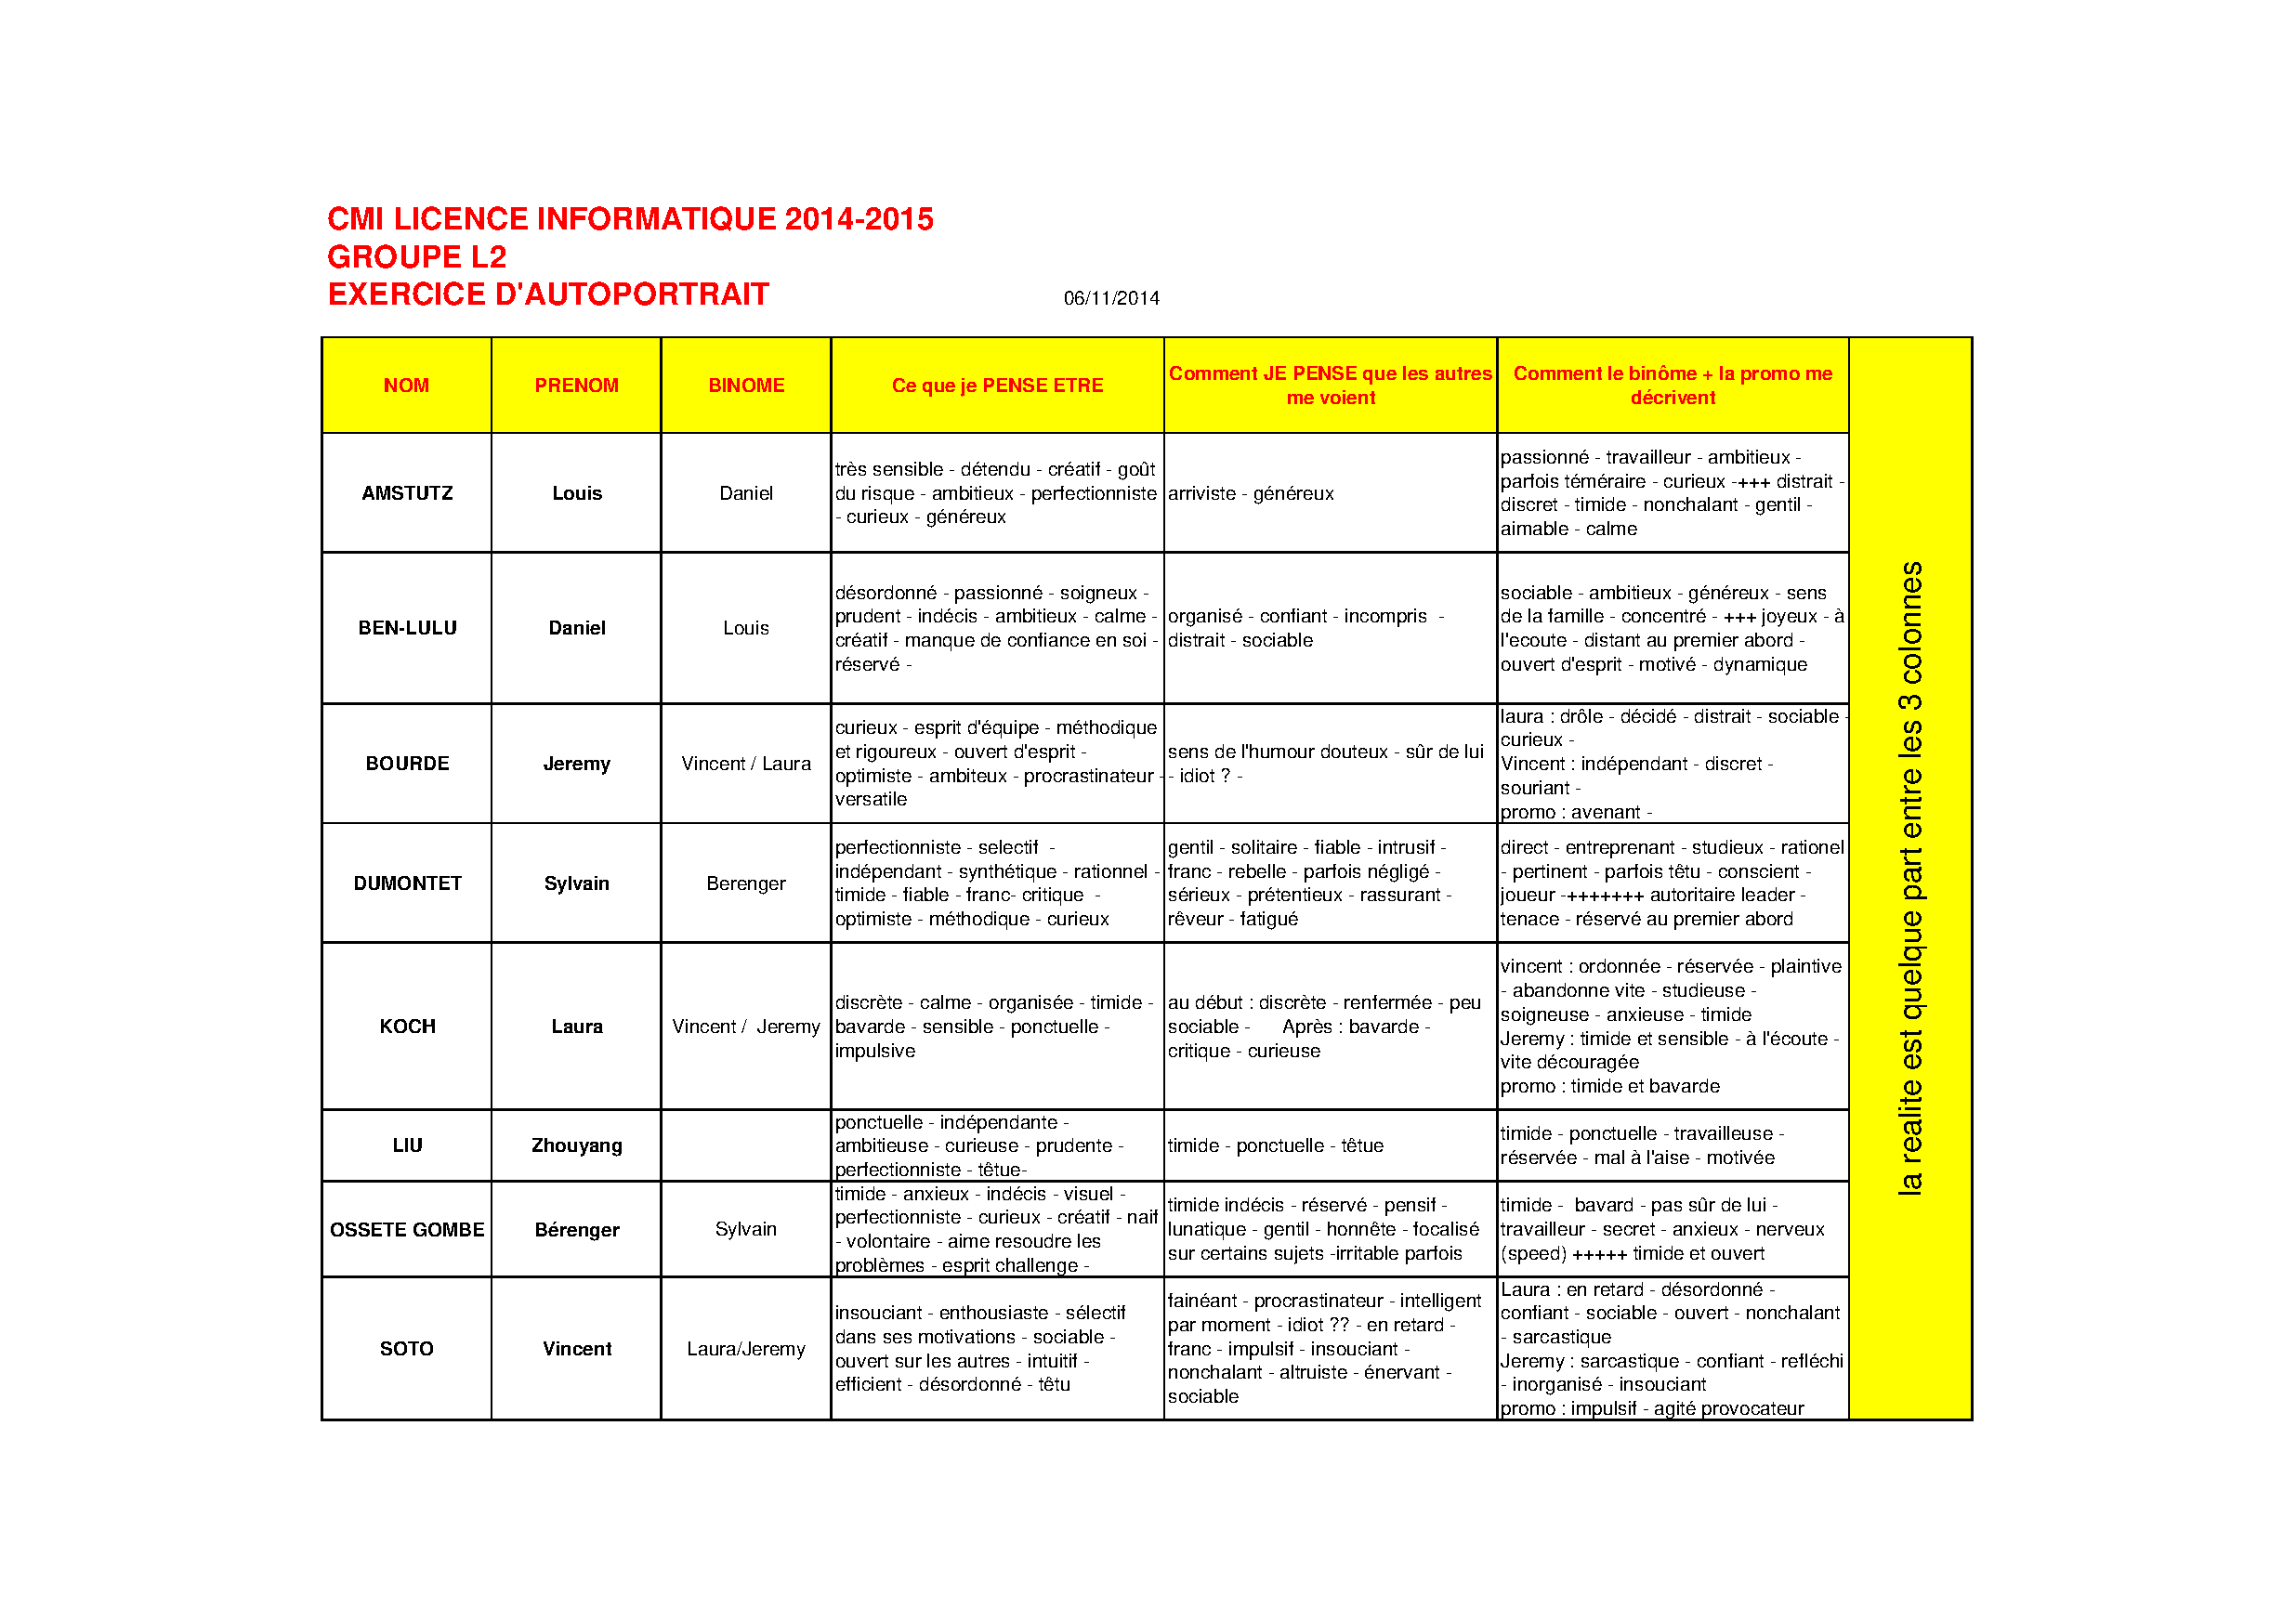
\includepdf[pages = 1]{autoportraitCMI.pdf}

\chapter{Interview de Chriswot en anglais}\label{chriswot_en}

\begin{description}
\item [Question]:  Hi ! Thank you !
\item [Réponse]:  What did you want to know ?
\item [Question]:  First i am a computer science student and I looking for information about free software dev. I want to work in that domain but I don't know what type of job exists with the free software philosophy.
\item [Réponse]:  It depends - to get paid to do free software you really need to find a place that is getting paid for support.
\item [Question]:  My first question would be: Who are you ? A libreoffice developer's ? (Can you introduce yourself ?)
\item [Réponse]:  I'm a LibreOffice developer who's about to take up a paid \\contract with Collabora. I've been working on LO for about a year now, on and off. Doing a lot of reading and refactoring. Getting to know folks on IRC gradually
\item [Question]:  For you which domain of computer science are the more concerned by the free software dev ?
\item [Réponse]:  Coding and testing. That's a big question ! Do you mean, what aspect of software am I interested in? Like application software, frameworks, operating systems, etc ?
\item [Réponse]:  Well, for now I am interested in application software, but that's a large area. I'm currently focusing on the widget layer of LO, called VCL
\item [Question]:  Can you explain me how did you step in the free software dev ?
\item [Réponse]:  I started by reading the code after seeing a post about LO on Hacker News
\item [Question]:  And what advices you would give to a student who wants to work in free software dev ?
\item [Réponse]:  For me, I looked for the entry point of LO (the main function). Then I traced through the code and eventually started making some small changes after working out how to setup the build tools. Sure, a big enough free software project takes time to understand. The very first thing is to work out how to get the source code, and work out how to build it. Then I'd read all the documentation you can find, and be prepared to do a LOT of code reading. Work out if there are any easy changes you can make, like typos in comments, silly mistakes that can be fixed. Make those changes then work out how to get those changes integrated into the core product. Some projects like LO make it easy (e.g. we use gerrit), other projects it's quite hard. Be prepared to write a document about what you find, even if you use it only for yourself. Lurk on IRC for a while and try to gradually ask questions and show you are working on issues, but if you ask a question on IRC on a dev channel, always explain that you have read the documentation and that it wasn't clear, could someone clarify otherwise you might be mildly flamed :-) . But above all, be prepared to take on feedback, and be prepared to go outside your comfort zone and learn how to use git properly :-)
\item [Question]:  what do you mind when you say " go outside your comfort zone" ?
\item [Réponse]:  Try stuff on your local machine - be willing to make mistakes. Look at areas you don't understand - sometimes you'll need to read up on odd things. For instance, I'm currently reading all the EMF specs from Microsoft so that I can get drawing in documents working. Don't be afraid to break stuff on your local workstation - if you branch code in git, it's very hard to go wrong as you can checkout the master branch and start a new branch.
\item [Question]:  Is LO development your main job ?
\item [Réponse]:  It will be shortly :-) but before this I've worked in a variety of jobs.
\item [Question]:  A variety of jobs in computer science 's field ?
\item [Réponse]:  More IT than computer science.
\item [Question]:  Did you work with free softwares ?
\item [Réponse]:  I was a support person, a senior software troubleshooter for a VMWare product, stuff like that. I did a few things. Not much really, but I helped troubleshoot some nasty bugs in Firefox. However, I've been involved in free culture projects, like Wikipedia. At one time at a reasonably influential level.
\item [Question]:  So now you need to have another job ? I  only want to work with free software. So the main issues is: what kind of jobs can I choose to get paid and to develop free software ?
\item [Réponse]:  Do you want to develop free software? Not many projects are monetized, but you can get roles being a sysadmin and contribute to free software.
\item [Question]:  Yes I would like to. I don't really know what is a sysadmin, can you explain me what does a sysadmin do ?
\item [Réponse]:  Looks after computer systems :-) server admin work normally. Basically, you need to find an itch and scratch it.
\item [Réponse]:  My interest was LO. There is no silver bullet, I'm getting paid because there is demand for my skills and I did a lot of dedicated work and proved my skills to the other developers over a long period of time.
\item [Question]:  So you work from home ?
\item [Réponse]:  Yep, I live in Australia and most of the rest of the devs in the company I work for are in Europe or in the UK.
\item [Question]:  Will you earn money when you will be working exclusively for LO ?
\item [Réponse]:  I might do some side jobs, the job only lasts for 2 months so far.
\item [Question]:  So you will always need to have side jobs ? In your sides jobs do you use free software ?
\item [Réponse]:  To be honest, this is my first paid gig as a free software developer, but I suspect that this will be the case. Then again, I have a lot of freedom in this role that I can't get at a normal workplace.
\item [Réponse]:  I can take my kids to school in the morning, do chores, no micro-managing, that sort of thing.
\item [Question]:  Do you have to change your side jobs frequently ?
\item [Réponse]:  Actually, I took on this role when I was made redundant. I got a good payout. Anyhow... I gotta get some coding done - hope I was helpful :-)
\item [Question]:  You were helpful :) thank you very much ! (And sorry for my bad english)
\item [Réponse]:  no probs :-) best of luck
\item [Réponse]:  not at all, you were fine :-)

\end{description}


%%%%%%%%BIBLIO-WEBOGRAPHIE
\renewcommand{\bibname}{Webographie} 

\begin{thebibliography}{12}
\bibitem{annuaire_ssll} http://www.linux-france.org/article/pro/annuaire/
\bibitem{cnll} http://www.cnll.fr/
\bibitem{lolix} http://fr.lolix.org/
\bibitem{apce} http://www.apce.com/pid648/cooperatives-activites.html
\bibitem{cnll_etude} http://www.cnll.fr/news/resultats-etude-2014/
\bibitem{linuxfr_new} https://linuxfr.org/users/lebouquetin/news
\bibitem{bountySource} https://www.bountysource.com/
\bibitem{fossFactory} http://www.fossfactory.org/
\end{thebibliography}

\end{document} 
 
 
